\section{Experimental Evaluation}
\label{sec:experiments}

The evaluation treats MouseClaimBench as a knowledge representation and inference system. It addresses logical completeness, false authorization under known structural truth, faithful inference over real mouse-brain artifacts, and behaviour under external substitution failures. It does not compare neural architectures or claim state-of-the-art performance on the external datasets.

\subsection{Protocol}
\label{subsec:experimental-protocol}

Logical evaluation starts when the profile is loaded. Tests reject duplicate or incomplete declarations and evaluate all $5^{4}=625$ state assignments for the four-block mechanistic claim. Expected decisions follow the declared precedence $F\succ R\succ U\succ N\succ P$. Additional tests cover undeclared claims, absent facts, index consistency, deterministic graph export, and equivalence with the frozen legacy interface.

The known-truth benchmark contains five \ac{sem} regimes: independence, common cause, $X\rightarrow Y$, $Y\rightarrow X$, and a direct relation with an explicit intervention. Each regime generates 100 independent cases with separate fitting, held-out, and internal-reproduction cohorts of 600 observations. The data-generating graph and intervention define the reference claims before MouseClaimBench receives finite-sample diagnostics for prediction, topology, direction, and intervention. The resulting 500 cases produce 5,000 claim decisions per policy.

The comparator is a prediction shortcut that promotes successful prediction to topology, direction, mechanism, and causality. We report \ac{fpr} and \ac{fnr} over decisions with descriptive Wilson intervals. The confirmatory comparison uses each generated case as one unit. Within-case error counts are compared by an exact two-sided sign test over non-tied cases, avoiding an independence assumption across the ten decisions from the same case.

Four artifact-grounded cases provide complementary evidence. Allen \ac{vbn} examines internal reproduction, topology controls, and directional identifiability. Static Sensorium evaluates held-out prediction and topographic specificity across five datasets. Dynamic Sensorium evaluates temporal prediction in two stored five-mouse cohorts. The local \ac{microns} case evaluates an observational structure--function endpoint in one cortical volume. Adapters retain source observations and execute source-specific predicates. A conformance audit rebuilds all four fact bases and compares the resulting ten claims per case with 40 frozen decisions. It also requires a fired rule, complete rule sequence, profile hash, and one preserved fact per required block.

SciFact and Tuebingen provide external failure controls for retrieval and causal direction \citep{wadden2020scifact,mooij2016cause}. Transparent SciFact baselines separate document retrieval from support authorization. Three direction proxies on 108 Tuebingen cause--effect pairs test whether association can satisfy direction. A legacy suite of 144 constructed cases remains regression evidence for component ablation and threshold perturbation. Its labels share the historical gate semantics, so it is not used as independent scientific validation. Detailed configurations, secondary tables, ablations, and sensitivity plots are supplied as Supplementary Material and as clean revision-bound artifacts.

\subsection{Logical and oracle results}
\label{subsec:oracle-results}

The profile passes all structural checks, and every mechanistic assignment reaches exactly one expected conclusion. Failure blocks support even when another fact requires review or is absent. Review, unknown, and not-applicable states remain distinct. The all-passed assignment is the only route to support. This establishes total deterministic execution for the tested claim, not completeness of the scientific taxonomy.

MouseClaimBench produces 1,954 \acp{tp}, 56 \acp{fp}, 2,844 \acp{tn}, and 146 \acp{fn}. Its \ac{fpr} is $0.0193$ with a descriptive 95\% Wilson interval of $[0.0149,0.0250]$, and its \ac{fnr} is $0.0695$ with interval $[0.0594,0.0812]$. The prediction shortcut produces 2,085 \acp{tp}, 785 \acp{fp}, 2,115 \acp{tn}, and 15 \acp{fn}, corresponding to an \ac{fpr} of $0.2707$ and an \ac{fnr} of $0.0071$. The knowledge policy therefore exchanges sensitivity for 729 fewer false authorizations under the declared regimes.

At case level, MouseClaimBench has fewer errors in 263 of 500 cases, the shortcut has fewer in 77, and 160 are tied. The exact sign-test value over 340 non-tied cases is $p=6.41\times10^{-25}$. Fig.~\ref{fig:oracle-benchmark} reports both error rates so that the increased conservativeness remains explicit. The result supports the policy under these five generators and does not establish optimality under arbitrary or biological dynamics.

\begin{figure}[t!]
\centering
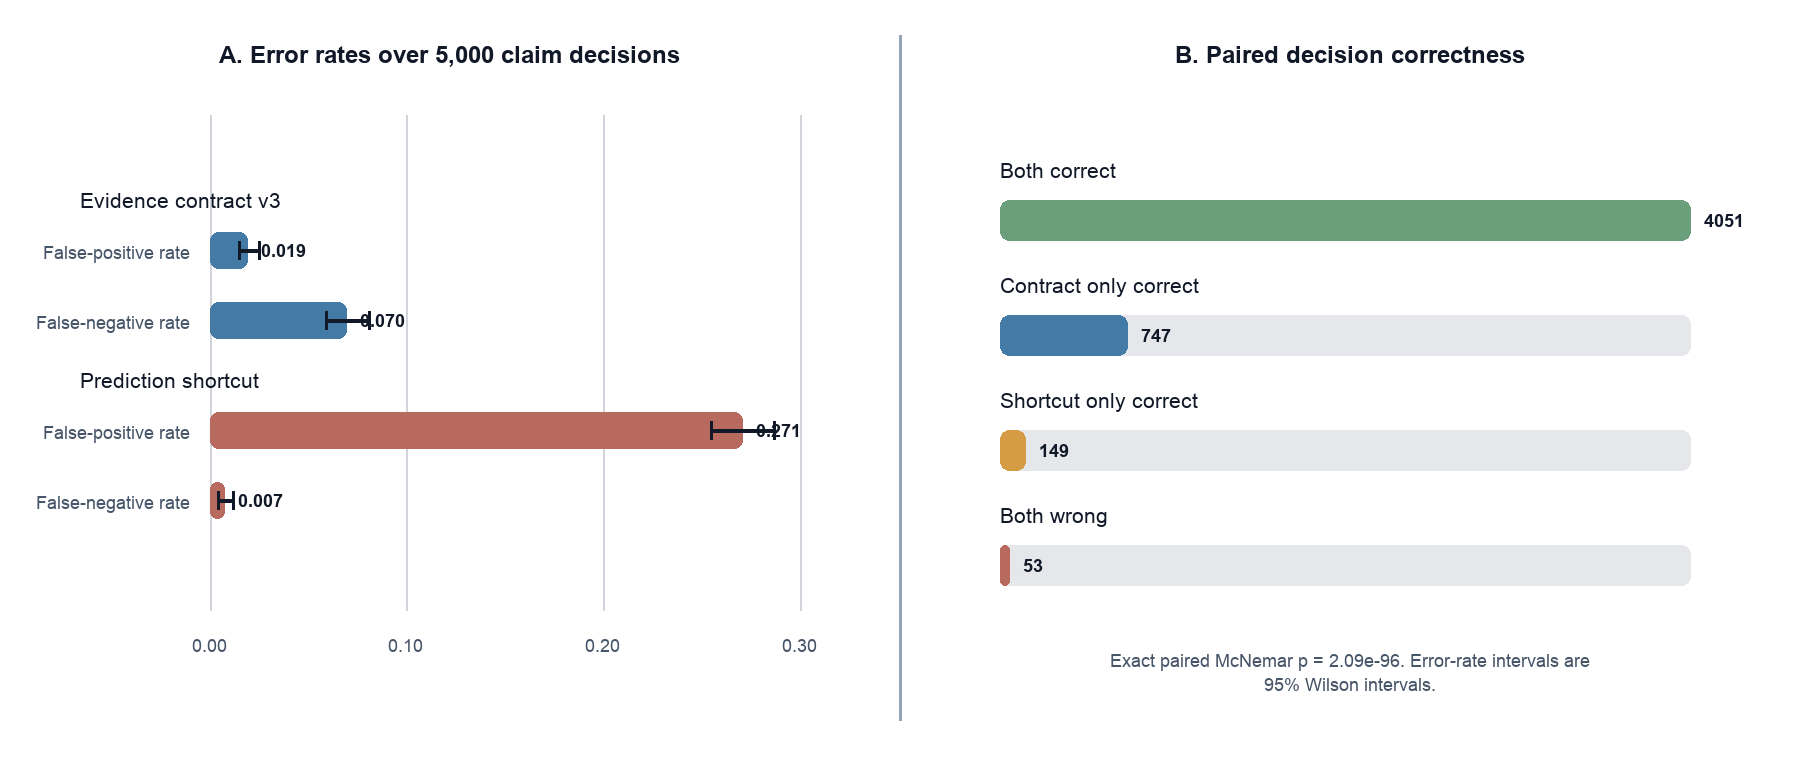
\includegraphics[width=0.96\textwidth]{figures/claimbench_oracle_benchmark.png}
\caption{Evaluation on the oracle structural-equation benchmark. Panel A reports
standard false-positive and false-negative rates with 95\% Wilson intervals over
5,000 claim decisions. Panel B compares correctness for the same decisions under
the non-compensatory contract and a prediction-only shortcut. Inferential
comparison uses the 500 generated cases as units rather than treating dependent
claim decisions within a case as independent. Reference labels
come from the declared data-generating graph and intervention availability,
whereas evidence statuses come from finite-sample diagnostics.}
\label{fig:oracle-benchmark}
\end{figure}


\subsection{Mouse-brain cases, controls, and release evidence}
\label{subsec:artifact-results}

The four real cases produce 10 supported, 7 blocked, 7 uncertain, and 16 out-of-scope decisions. None supports external replication, causality, or a complete digital twin. Fig.~\ref{fig:real-case-matrix} displays all 40 dispositions. The complete observation-to-decision table is provided in the Supplementary Material.

\begin{figure}[t!]
\centering
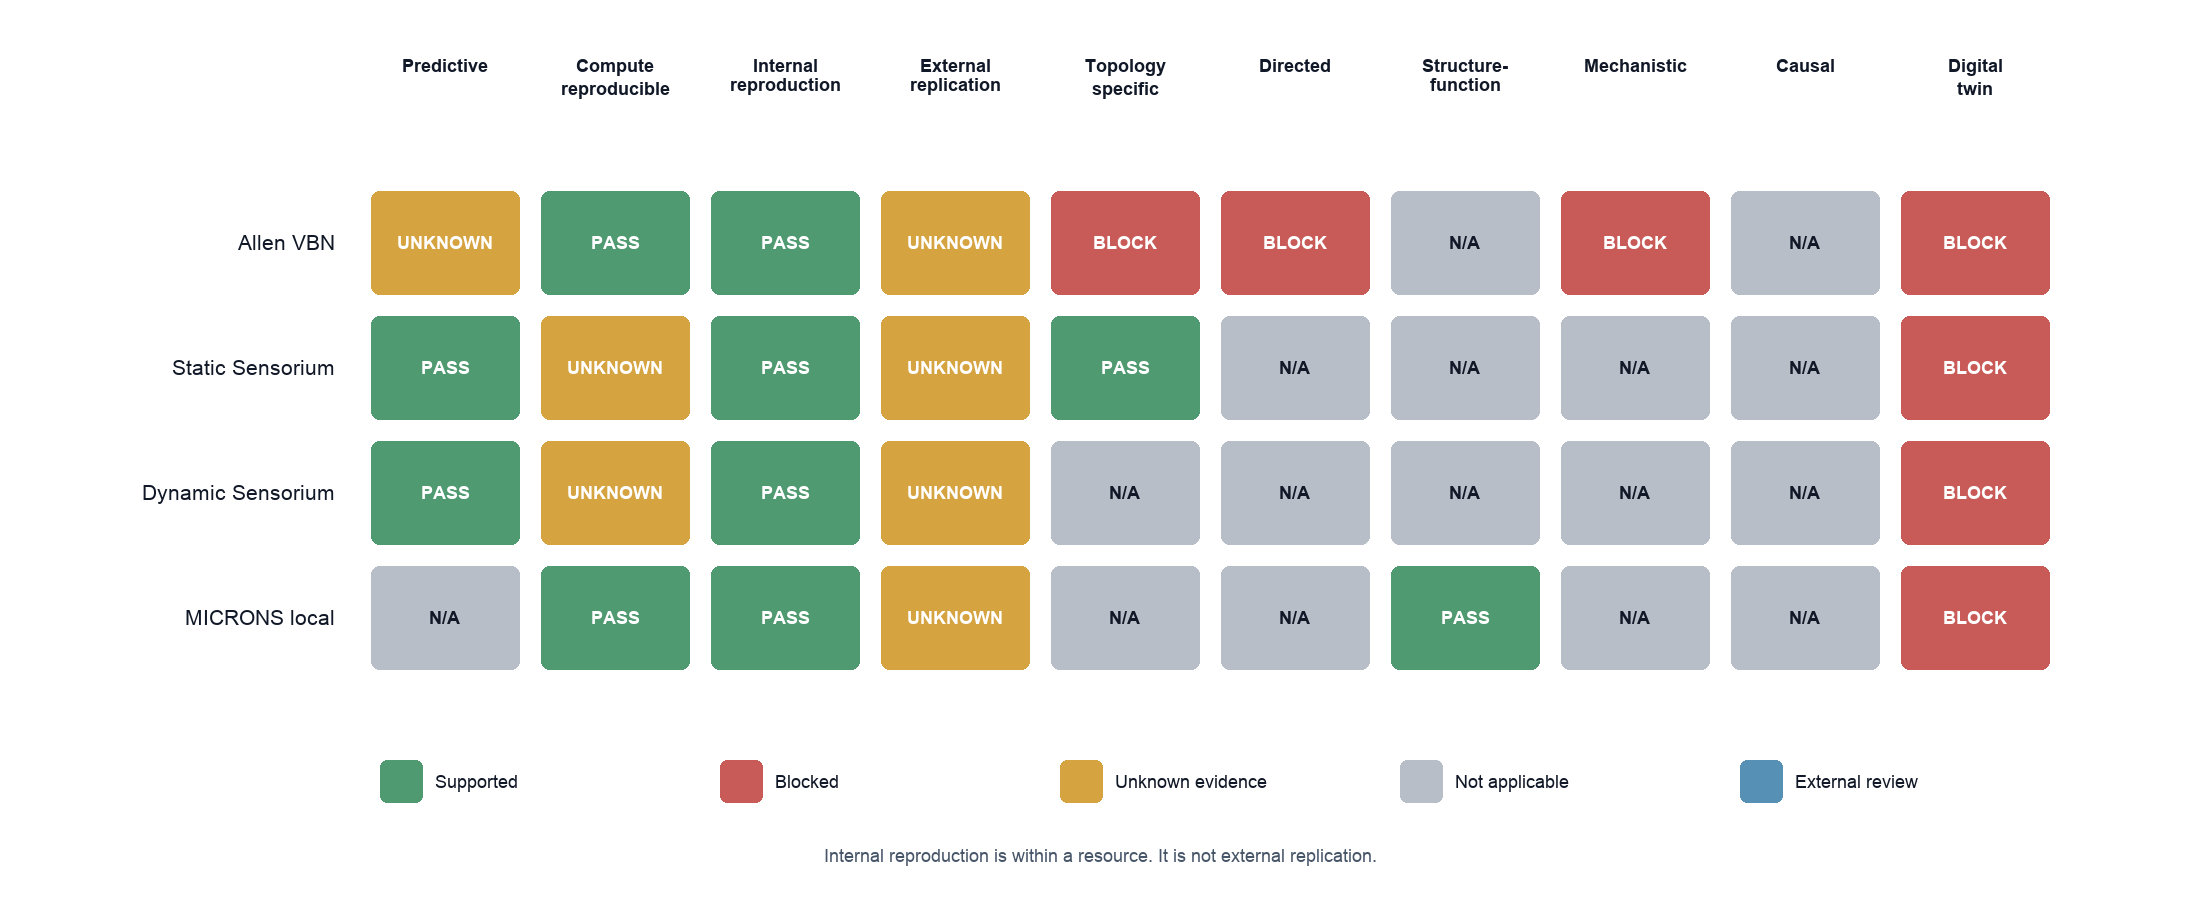
\includegraphics[width=0.98\textwidth]{figures/claimbench_real_case_matrix.png}
\caption{Forty artifact-grounded decisions for four mouse-brain cases. Each cell
has a fired rule, source facts, and a proof trace. Unknown denotes missing
evidence, while not applicable denotes an untargeted protocol. Internal
reproduction uses non-overlapping units or cohorts within one resource and is
not external replication.}
\label{fig:real-case-matrix}
\end{figure}


Allen is a negative mechanistic case despite strong internal reproduction. Median cross-mouse and split-half correlations are $0.891$ and $0.990$, but topology performs $-0.0054$ below the median permutation, its bootstrap lower bound is $-0.0075$, and all six direction criteria equal zero. Static Sensorium supports prediction and topology in five datasets, with median predictive correlation $0.341$ and positive gains over mean and scrambled baselines. Dynamic Sensorium supports temporal prediction and internal reproduction, with temporal \ac{svd} exceeding the mean-response baseline in 4/5 and 5/5 mice across the stored comparisons. Neither Sensorium case supplies intervention, external replication, or biological directional identification.

The \ac{microns} endpoint was fixed after discovery and evaluated in two non-overlapping hold-out windows. Discovery contains 1,000 units and 2,095 connected directed pairs. The hold-outs contain 992 and 999 units with 1,926 and 1,922 pairs. Distance-matched deltas are $0.0215$, $0.0210$, and $0.0179$, with positive unit-cluster weighted bootstrap lower bounds. Degree-matched deltas are also positive in all windows. This supports a local observational structure--function association, not causality, external replication, or whole-brain coverage.

The conformance audit exactly reproduces all 40 frozen decisions and provides 40 complete traces. The operational graph contains 36 nodes and 45 edges. SciFact further shows that a train-calibrated policy can reduce \ac{fpr} to $0.068$ on 300 development claims while increasing \ac{fnr} to $0.718$. Tuebingen direction accuracy is $0.485$ over 103 attempted pairs, with a 95\% Wilson interval of $[0.391,0.581]$. These controls block the substitutions of retrieval for support and association for causal direction.

The legacy ablations reproduce all 1,152 expected decisions. Removing topology or direction introduces 12 false authorizations in each case, while a compensatory score introduces 84 false authorizations and 75 false rejections. The release gate verifies nine artifact families, the profile hash, all frozen decisions and traces, and clean Git revisions. Its passing state establishes package consistency only. Cross-domain generality, external biological replication, improved human outcomes, and complete causal digital-twin scope remain explicitly blocked.
